%!TEX TS-program = xelatex
%!TEX encoding = UTF-8 Unicode

\documentclass{harvard-thesis}



\usepackage{tikz}

\usepackage{textcomp}
\usepackage{gb4e}

\usepackage{multirow}

\begin{document}

% the front matter
% some details about the thesis
\title{A Concise Grammar of Ishiculu}
\author{Ming Zhang}
\advisor{Dr. Allison Biggs}

% about the degree
%\degree{Doctor of Philosophy}
%\field{LING }
\course{LING 242}
\degreeyear{$\rule[0.5ex]{2em}{0.1ex}\hspace{-2em}\text{2017}$\ \ 2117}
\degreemonth{December}

% about the university
%\department{Department}
\university{University of Pennsylvania}
\universitycity{Philadelphia}
\universitystate{Pennsylvania}
\maketitle
%\copyrightpage
%\abstractpage
\tableofcontents
%\authorlist
%\listoffigures
%\dedicationpage
%\acknowledgments

\onehalfspacing

% incluude each chapter...

\chapter{Demographics and ethnographics}

\newthought{Ishiculu is a creole language} spoken by the Kuxutshwe, a community in KwaZulu-Natal, South Africa of people of mixed Zulu and Chinese ancestry. The term ``Kuxutshwe'' means ``mixed'' in Zulu, and is the self-referent of the Kuxutshwe people.

Before the 2020s, there had been American scholars and organizations in eastern South Africa building health infrastructure. This trend motivated other organizations, mostly from the Greater China Region, to add to their presence in eastern South Africa. By the end of the 2020s, because of a strengthened South African government and a pivot of US international policies, most Americans set out to contribute to cross-nation collaborations had left. In 2034, a private corporation from Taiwan discovered an oil well just off Richards Bay, a town in KwaZulu-Natal, South Africa. This incentivized more Chinese people to reside in eastern South Africa, and a community of Ishiculu speakers descended from a mixture of Zulu and Chinese people. By 2105, Ishiculu had about 1500 speakers in KwaZulu-Natal.

Ishiculu is now mostly spoken in KwaZulu-Natal near the east coast. In these communities where Ishiculu is spoken, Zulu and Chinese are usually also used. The Kuxutshwe people usually live and engage in social interactions with Zulu and Chinese people. Both Chinese and Ishiculu have seen a slight decrease in the number of speakers since the 2080s, a fact possibly attributed partially to their lack of legal status. There has been some but insufficient literature on marginalization of the Kuxutshwe people in both Zulu- and Chinese-speaking communities, but the existing research has indicated that the interactions between Ishiculu speakers and other peoples are mostly friendly and social, and that the marginalization stems from the way local educational and legal systems are set up. The major languages spoken in KwaZulu-Natal is listed in Table 1, and the racial makeup of Richards Bay is shown in Table 2.

\begin{table}
\centering
\begin{tabular}{l|l}
Zulu & 71.8\% \\
\hline
English & 15.2\% \\
\hline
Xhosa & 4.4\% \\
\hline
Afrikaans & 2.6\% \\
\hline
Ishiculu & $<$ 0.01\%
\end{tabular}
\caption{Major languages spoken in KwaZulu-Natal (2105)}
\end{table}

\begin{table}
\centering
\begin{tabular}{l|l}
Black African & 43.0\% \\
\hline
Coloured (Including Kuxutshwe) & 4.2\% \\
\hline
Indian/Asian & 19.2\% \\
\hline
White & 33.1\% \\
\hline
Other & 0.4\%
\end{tabular}
\caption{Racial makeup of Richards Bay (2101)}
\end{table}

\begin{figure}
\begin{tikzpicture} 
    \node[anchor=south west,inner sep=0] (image) at (0,0) {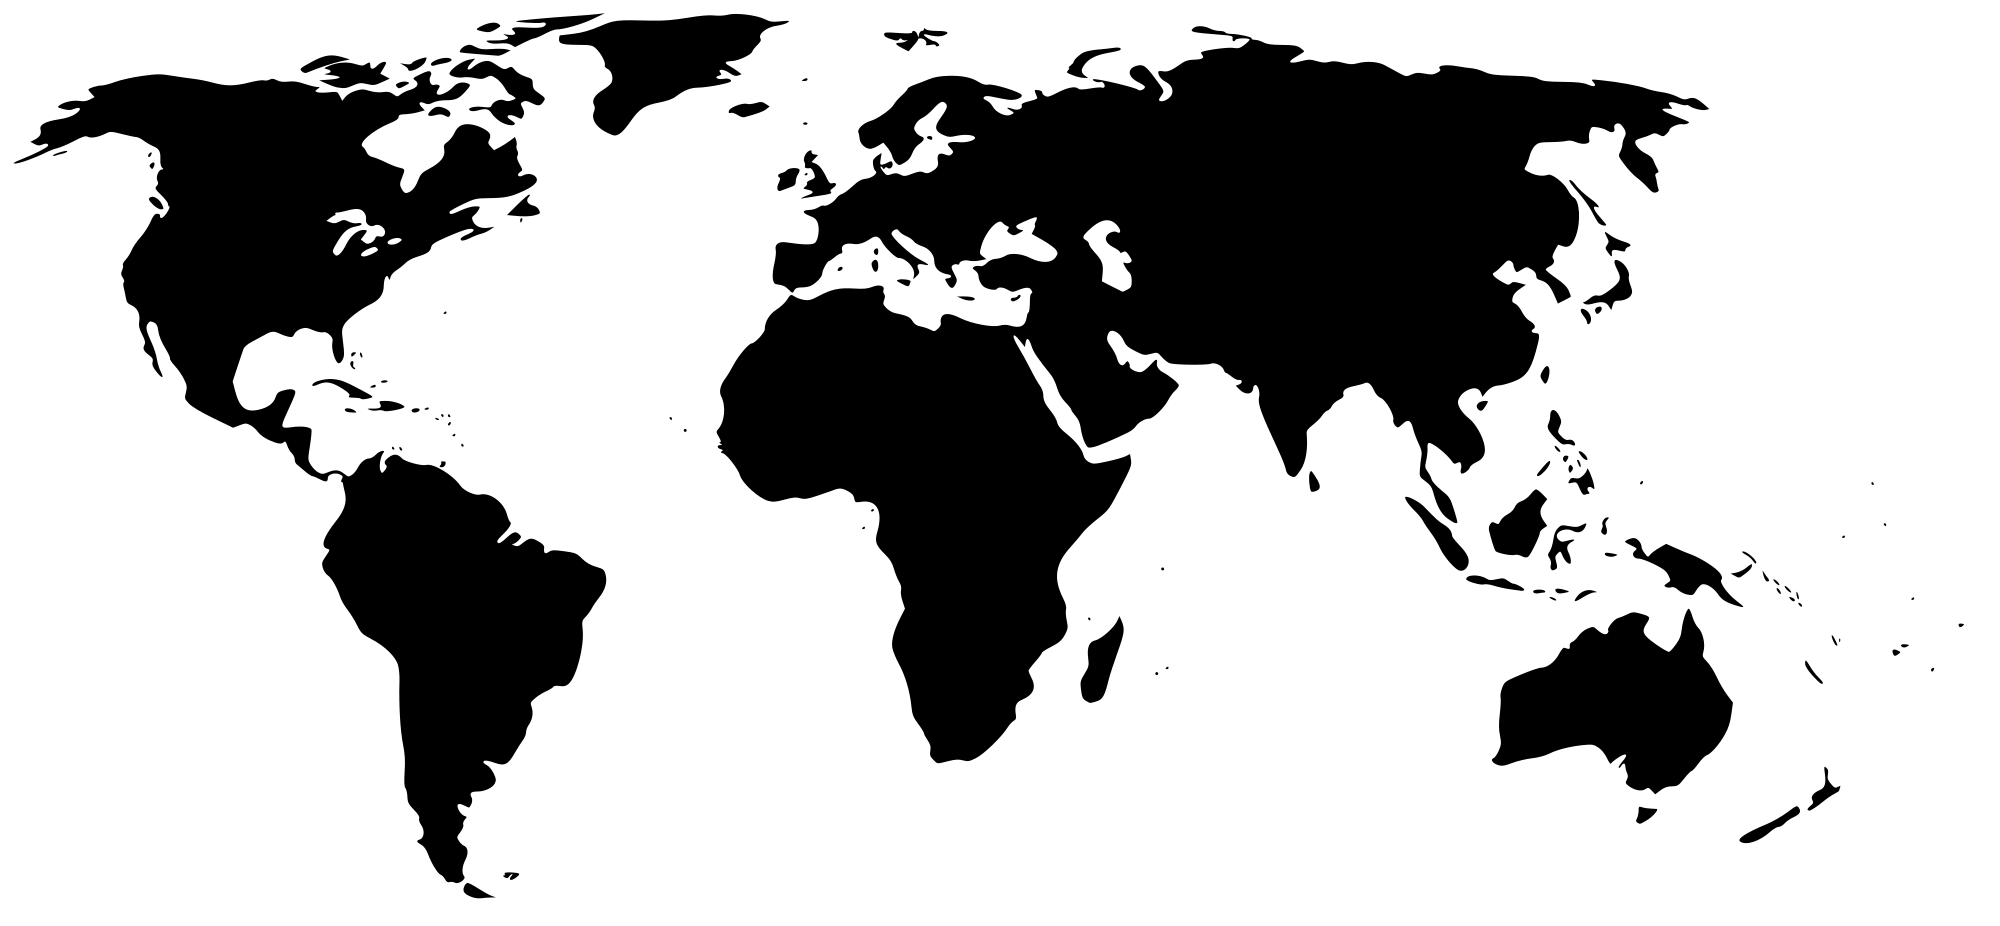
\includegraphics[width=1\textwidth]{figures/world-map.png}};
    \begin{scope}[x={(image.south east)},y={(image.north west)}]
        \draw[->,red,ultra thick] (0.755,0.605) to [out=180,in=60] (0.49,0.22);
    \end{scope}
\end{tikzpicture}
\caption{Migration of Chinese people to South Africa in the 2030s}
\end{figure}
\chapter{Phonology}

\section{Phoneme inventory}

\newthought{There are 31 consonants} and six vowels in Ishiculu, shown in Table~\ref{table:phonology:consonant-chart} and Figure~\ref{fg:phonology:vowel-space}. This consonant-vowel ratio is considered moderately high crosslinguistically \cite{wals-3}.

\begin{table}
\centering
\begin{tabular}{|l|l|c|c|c|c|c|}
\hline
\multicolumn{2}{|c|}{} &
Labial &
Alveolar &
Postalveolar &
Palatal &
Velar \\

\hline
\multirow{3}{*}{Stop} & voiced &
b & \multicolumn{2}{c|}{d} & & \textipa{g} \textlangle g\textrangle \\

\cline{2-7}
 & voiceless &
p & \multicolumn{2}{c|}{t} & & k \\

\cline{2-7}
 & aspirated &
\raisebox{-1pt}{p\textipa{\super h}\ \textlangle ph\textrangle} & \multicolumn{2}{c|}{\raisebox{-1pt}{t\textipa{\super h}\ \textlangle th\textrangle}} & & \raisebox{-1pt}{k\textipa{\super h}\ \textlangle kh\textrangle} \\

\hline
\multicolumn{2}{|l|}{Nasal} &
m & \multicolumn{2}{c|}{n} & \textltailn\ \textlangle gn\textrangle & \textipa{N}\ \textlangle ng\textrangle \\

\hline
\multicolumn{2}{|l|}{Trill} &
& \multicolumn{2}{c|}{r} & & \\

\hline
\multirow{2}{*}{Fricative} & voiced &
& & \textipa{Z}\ \textlangle zh\textrangle & & \textipa{G}\ \textlangle gh\textrangle \\

\cline{2-7}
& voiceless &
f & s & \textipa{S}\ \textlangle sh\textrangle & & x \textlangle h\textrangle \\

\hline
\multirow{2}{*}{Affricate} & voiced &
& \raisebox{-1.5pt}{\textipa{\t{dz}}} \textlangle dz\textrangle & \raisebox{-1.5pt}{\textipa{\t{dZ}}} \textlangle j\textrangle & & \\

\cline{2-7}
& voiceless &
& \raisebox{-1.5pt}{\textipa{\t{ts}}} \textlangle ts\textrangle & \raisebox{-1.5pt}{\textipa{\t{tS}}} \textlangle ch\textrangle & & \\

\hline
\raisebox{-2pt}{Lateral} & voiced &
& \multicolumn{2}{c|}{\textlyoghlig} & & \\

\cline{2-7}
\raisebox{1pt}{fricative} & voiceless &
& \multicolumn{2}{c|}{\textbeltl} & & \\

\hline
\multicolumn{2}{|l|}{Approximant} &
\textipa{V} & \multicolumn{2}{c|}{} & j \textlangle y\textrangle & w \\

\hline
\multicolumn{2}{|l|}{Lateral approximant} &
& \multicolumn{2}{c|}{l} & & \\

\hline
\multicolumn{2}{|l|}{Click} &
& \multicolumn{2}{c|}{\textipa{\super N|} \textlangle c\textrangle} & & \\

\hline
\end{tabular}
\caption{Phonemic consonants in Ishiculu. Letters in angle brackets represent the phonemes in Ishiculu orthography.}
\label{table:phonology:consonant-chart}
\end{table}

\begin{figure}
\centering
\begin{vowel}
\putcvowel{i}{1}
\putcvowel{\textipa{E}\ \textlangle e\textrangle }{3}
\putcvowel{a}{4}
\putcvowel{\textipa{O}\ \textlangle o\textrangle }{6}
\putcvowel{\textipa{7}}{7}
\putcvowel{u}{8}
\end{vowel}
\caption{Phonemic vowels in Ishiculu. Letters in angle brackets represent the phonemes in Ishiculu orthography.}
\label{fg:phonology:vowel-space}
\end{figure}

\section{Syllable structure}
Possible syllable structures in Ishiculu are (C)V and N\textsubscript 1C\textsubscript 1V, where N\textsubscript 1 is a nasal with the same place of articulation as obstruent C\textsubscript 1. Some examples of syllabification are shown in Example~\ref{ex:phonology:syllabification}.

\ 
\\

\begin{exe}
\ex Syllabification in Ishiculu
\begin{xlist}
\ex \textlangle Ishiculu\textrangle \quad /\textipa{i.Si.\super N|u.lu}/ \quad V.CV.CV.CV
\ex \textlangle unjani\textrangle \quad /\textipa{u.\textltailn\t{dZ}a.ni}/ \quad V.NCV.CV
\end{xlist}
\label{ex:phonology:syllabification}
\end{exe}

As a lexically tonal language, it's uncommon for Ishiculu to have no coda. Mandarin and Cantonese both have some simple codas and lexical tones. The lexical tones survived, but the codas did not. On the other hand, Zulu has no coda and only grammatical tones. 

\section{Tones and stress}

\subsection{Tonemes}

Ishiculu has four tones, shown in Table~\ref{table:phonology:tones}. Note that the tones are not indicated in Ishiculu orthography.

\begin{table}[H]
\centering
\begin{tabular}{|l|c|c|c|c|}
\hline
Description & low & high & rising & falling \\
\hline
IPA diacritic & \textipa{\`a} & \textipa{\'a} & \textipa{\v a} & \textipa{\^a} \\
\hline
Tone contour & 11 & 55 & 35 & 51 \\
\hline
\end{tabular}
\caption{Tonemes in Ishiculu.}
\label{table:phonology:tones}
\end{table}

\subsection{Interactions between voiced stops and tones}

Voiced stops in Ishiculu (i.e. /b/, /d/, and /\textipa g/) add a low-tone onset to the normal tone.

\begin{table}[H]
\centering
\begin{tabular}{|l|c|c|c|c|}
\hline
Normal tone & \textipa{\`a} (low) & \textipa{\'a} (high) & \textipa{\v a} (rising) & \textipa{\^a} (falling) \\
\hline
New tone & \textipa{b\`a} (low) & \textipa{b\v a} (rising) & \textipa{b\v a} (rising) & \textipa{b\textrisefall{a}} (rising-falling) \\
\hline
\end{tabular}
\caption{Tone change after voiced stops.}
\end{table}

\subsection{Stress}
The stress of an Ishiculu word falls on the penultimate syllable and results in lengthening of the vowel. Some examples are shown in (\ref{ex:phonology:stress}).
\begin{exe}
\ex
\begin{xlist}
\ex \textlangle Ishiculu\textrangle \quad /\textipa{i.Si.\super N|u.lu}/ \quad [\textipa{iSi\super N|u:lu}]
\ex \textlangle unjani\textrangle \quad /\textipa{u.\textltailn\t{dZ}a.ni}/ \quad [\textipa{u\textltailn\t{dZ}a:ni}]
\end{xlist}
\label{ex:phonology:stress}
\end{exe}

\chapter{Constituent order}

\section{Basic word order}
\newthought{Ishiculu is subject-prominent}, with a basic word order of SVO.

\begin{exe}
\ex
\gll Ari pa ka-shiy-ioani nta\textbeltl o kitabu. \\
Ari not \textsc{1.sg}-\textsc{7.sg}-like \textsc{clf}.7 book(7) \\
\trans `Ari doesn't like the book.'
\ex
\gll Shi-shiy-ioani-mbi nta\textbeltl o kitabu. \\
\textsc{1pl}-\textsc{7.sg}-like-\textsc{pst} \textsc{clf}.7 book(7) \\
\trans `We used to like the book.'\ex
\gll Fu Philadelphia shi-ka-shi-ke-\textbeltl a Ari nta\textbeltl o kitabu. \\
\textsc{prep.int} Philadelphia \textsc{1pl}-\textsc{1.sg}-\textsc{7.sg}-have-\textsc{caus} Ari \textsc{clf}.7 book(7) \\
\trans `We will give Ari the book in Philadelphia.'
\end{exe}

Sometimes in Ishiculu, the predicate position can be filled by an uninflected adjectival phrase, such as an adjective or an adpositional phrase.

\begin{exe}
\ex
\gll Ari fu Philadelphia tso. \\
Ari \textsc{prep.int} Philadelphia \textsc{post.abl} \\
\trans `Ari is from Philadelphia.'
\ex
\gll Ari \textbeltl o\textbeltl o. \\
Ari small \\
\trans `Ari is little.'
\end{exe}

\subsection{Locative expression}
A locative phrase can occupy the subject position of an intransitive verb of existence or movement while the subject is then moved to the object position.

\begin{exe}
\ex
\gll {Ts\textramshorns} nta\textbeltl o nji tso \textbeltl i-huma nta\textbeltl o ika. \\
\textsc{prep.sur} \textsc{clf.7} table(7) \textsc{post.abl} \textsc{6.sg}-jump \textsc{clf}.6 cat(6) \\
\trans `Off the table jumps a cat.'
\ex
\gll Fu nta\textbeltl o heje shi-paka a\textlyoghlig o ntoch\textramshorns. \\
\textsc{prep.int} \textsc{clf.7} courtyard(7) \textsc{8.sg}-park \textsc{clf}.8 car(8) \\
\trans `In the courtyard is parked a car.'
\end{exe}

\subsection{Topicalization}
Topicalization can be carried out on the object to put emphasis, but a classifier for the object needs to remain in the post-verbal position.

\begin{exe}
\ex
\gll Kitabu shi-shi-so-mbi \textit{nta\textbeltl o}. \\
book(7) \textsc{1pl}-\textsc{7.sg}-read-\textsc{pst} \textsc{clf}.7 \\
\trans `The book, we have read it.'
\ex
\gll {Ntoch\textramshorns} ngi-shiy-ioani \textit{a\textlyoghlig o}. \\
car(8) \textsc{1sg}-\textsc{8.sg}-like \textsc{clf}.8 \\
\trans `The car, I like it.'
\end{exe}

\section{Modifiers of noun}

When demonstrative and/or numeral modify a noun, they always precede the noun. If they both modify the same noun, they are also found in this order. This particular word order is not uncommon among world's languages \cite{Greenberg-1963}. When a numeral modifies a noun, a classifier must also be used, which directly precedes the noun. See Chapter~\ref{ch:classifiers}.

\begin{exe}
\ex
\gll laba nta\textbeltl o kitabu \\
these \textsc{clf.7} book(7) \\
\trans `these books'
\ex
\gll a\textlyoghlig o {ntoch\textramshorns} \\
\textsc{clf.8} car(8) \\
\trans `the car(s)'
\ex
\gll nta nta\textbeltl o kitabu \\
three \textsc{clf.7} book(7) \\
\trans `three books'
\ex
\gll laba nta nta\textbeltl o kitabu \\
these three \textsc{clf.7} book(7) \\
\trans `these three books'
\end{exe}

An attributive adjective or a genitive follows the noun it modifies.

\begin{exe}
\ex
\gll {ntoch\textramshorns} caca \\
car big \\
\trans `big car(s)'
\ex
\gll nta\textbeltl o kitabu ce-mama \\
\textsc{clf.7} book(7) \textsc{gen}-mother \\
\trans `mother's book(s)'
\ex
\gll Fu u conkei \textbeltl oko shi-ka-shi-ke-\textbeltl a Ari nta nta\textbeltl o kitabu ce-Mel. \\
\textsc{prep.int} \textsc{clf.4} house(4) 4-red \textsc{1pl}-\textsc{1.sg}-\textsc{7.sg}-have-\textsc{caus} Ari three \textsc{clf}.7 book(7) \textsc{gen}-Mel \\
\trans `We will give Ari Mel's three books in the red house.'
\end{exe}

Example~\ref{ex:consitituent-order:all-modifiers} illustrates the ordering of all types of modifiers and adpositions with the same noun.

\begin{exe}
\ex
\glll fu laba nta u conkei caca ce-John tso \\
\textsc{prep.int} these three \textsc{clf.4} house big \textsc{gen}-John \textsc{post.abl} \\
Preposition Demonstrative Numeral Classifier \textbf{Noun} Adjective Genitive Postposition \\
\trans `out of these three big houses of John'
\label{ex:consitituent-order:all-modifiers}
\end{exe}
\chapter{Verbs}

\section{Agreements}

\newthought{Ishiculu exhibits highly synthetic} verbal morphology. In this sense, it is predominantly head-marking. Prefixation and suffixation are responsible for marking the agreements and the tense. Ishiculu is mostly agglutinative in terms of its verb affixation: different grammatical features of the verb are expressed through different affixes, except for the person and the number, which are contained in the same prefix. There are both inflectional and derivational verb affixes in Ishiculu.

The Ishiculu verb is marked according to a nominative-accusative alignment system. The verb stem is inflected based on the person, number, and, for 3rd person nominal phrases, the noun class. The structure of an inflected Ishiculu verb consists of nominative agreement, dative agreement, accusative agreement, stem, derivational suffixes, and tense, in this order. The same set of prefixes, shown in Table~\ref{table:verbs:personal-prefixes}, is used for all three agreements.

\begin{exe}
\ex
\gll \textit{Shi-shiy-ioani} \textipa{nta\textbeltl o} kitabu. \\
\textsc{1pl}-\textsc{cl7.sg}-like \textsc{clf}.7 book(7) \\
\trans `We (will) like the book.'
\ex
\gll Ari pa \textit{ka-uw-ioani} shidzi. \\
Ari not \textsc{cl1.sg}-\textsc{cl4.sg}-like cheese(4) \\
\trans `Ari doesn't like cheese.'
\end{exe}

\begin{table}
\centering
\begin{tabular}{c|c|c|c|c}
\hline
\multirow{2}{*}{} & \multicolumn{2}{c|}{singular} & \multicolumn{2}{c}{plural} \\
\cline{2-5}
 & before C & before V & before C & before V \\
\hline
\hline
1st person & -ngi- & -ngiw- & -shi- & -shiy- \\
\hline
2nd person & -u- & -uw- & -ni-& -niy- \\
\hline
CL 1/2 & \multicolumn{2}{c|}{-ka-} & \multicolumn{2}{c}{-ba-} \\
\hline
CL 3/4 & -u- & -uw- & -i- & -iy- \\
\hline
CL 5/6 & -\textbeltl i- & -\textbeltl iy- & \multicolumn{2}{c}{-a-} \\
\hline
CL 7/8 & -shi- & -shiy- & -\textipa{Z}i- & -\textipa{Z}iy- \\
\hline
\end{tabular}
\caption{Personal agreement prefixes of Ishiculu verbs.}
\label{table:verbs:personal-prefixes}
\end{table}

\section{Tenses}

Ishiculu has two tenses: present and past. The present tense is marked with a \textit{-\o} suffix, and can be used for future events. The past tense is marked with suffix \textit{\textipa{-mbi}}.

\begin{exe}
\ex
\gll Shi-shiy-ioani-\textit{mbi} \textipa{nta\textbeltl o} kitabu. \\
\textsc{1pl}-\textsc{cl7.sg}-like-\textsc{pst} \textsc{clf}.7 book(7) \\
\trans `We used to like the book.'
\end{exe}

\section{Imperative}

The imperative can occur either alone or with an object prefix, using one of the imperative suffixes shown in Table~\ref{table:verbs:imperative}.

\begin{table}
\centering
\begin{tabular}{c|l|l}
\hline
& \multicolumn{1}{c|}{Alone} & \multicolumn{1}{c}{With object} \\
\hline
Singular & \textit{-a} & \textit{-e} \\
\hline
Plural & \textit{-ani} & \textit{-eni} \\
\hline
\end{tabular}
\caption{Imperative suffixes in Ishiculu.}
\label{table:verbs:imperative}
\end{table}

\begin{exe}
\ex
\gll So-a! \\
read-\textsc{imp} \\
\trans `Read!'
\ex
\gll Shi-so-e \textipa{nta\textbeltl o} kitabu! \\
\textsc{cl7.sg}-read-\textsc{imp} \textsc{clf}.7 book(7) \\
\trans `Read the book!'
\end{exe}

\section{Valency-changing processes}
\subsection{Passive}

Morphological passive in Ishiculu is marked with \textit{\textipa{-wal7}} and decreases the valency of transitive verbs.

\begin{exe}
\ex
\gll U {-bon\textramshorns} -\textit{\textipa{wal7}} -mbi. \\
\textsc{2sg} -see -\textsc{pass} -\textsc{pst}  \\
\trans `You were seen.'
\ex
\gll Nta\textbeltl o kitabu shi-so-\textit{\textipa{wal7}}-mbi. \\
\textsc{clf}.7 book(7) \textsc{cl7.sg}-read-\textsc{pass}-\textsc{pst}  \\
\trans `The book was read.'
\end{exe}

The agent of the verb is then ineffable in the passive construction.

\ 
\\

\begin{exe}
\ex
\gll * Nta\textbeltl o kitabu shi-ngi-so-\textipa{wal7}-mbi mina. \\
{} \textsc{clf}.7 book(7) \textsc{cl7.sg}-\textsc{1sg}-read-\textsc{pass}-\textsc{pst} \textsc{pron.1sg} \\
\trans Intended meaning: `The book was read by me.'
\end{exe}

\subsection{Impersonal}
When the verb is impersonal, it does not bear a subject agreement prefix. The commonest impersonal is meteorological predicates.

\begin{exe}
\ex
\gll Cofi ha-mbi. \\
yesterday rain-\textsc{pst} \\
\trans `It rained yesterday.'
\end{exe}

Impersonal construction is also used for indefinite subjects. Note that this decreases the valency of the verb.

\begin{exe}
\ex
\begin{xlist}
\ex
\gll Pa ngi-shi-so nta\textbeltl o kitabu. \\
not \textsc{1sg}-\textsc{cl7.sg}-read \textsc{clf}.7 book \\
\trans `I don't/won't read the book.'
\ex
\gll Pa shi-so nta\textbeltl o kitabu. \\
not \textsc{7}-read \textsc{clf}.7 book \\
\trans `One doesn't/shouldn't read the book.'
\end{xlist}
\end{exe}

\subsection{Causative}

The suffix \textit{-\textbeltl a} marks the morphological causative form of a verb. Accordingly, as the valency of the verb is increased, the causee of the causative verb is marked as dative agreement on the verb.

\begin{exe}
\ex
\gll Ngi-ka-shi-so-\textbeltl a Ari \textipa{nta\textbeltl o} kitabu. \\
\textsc{1sg}-\textsc{cl1.sg}-\textsc{cl7.sg}-read-\textsc{caus} Ari \textsc{clf}.7 book(7) \\
\trans `I (will) make Ari read the book.'
\end{exe}

\subsubsection{Ditransitive}

Prototypical verbs in Ishiculu are transitive at most, and events that semantically require three core thematic arguments are expressed through causatives of transitive verbs.

\begin{exe}
\ex
\gll Fu Philadelphia ngi-ka-shi-ke-\textbeltl a Ari \textipa{nta\textbeltl o} kitabu. \\
\textsc{prep.int} Philadelphia \textsc{1sg}-\textsc{cl1.sg}-\textsc{cl7.sg}-have-\textsc{caus} Ari \textsc{clf.7} book(7) \\
\trans `I (will) give Ari the book in Philadelphia.'
\ex
\gll {W\textramshorns} babamama ba-ngiw-u-nde-\textbeltl a-mbi mina shizi. \\
\textsc{clf.2} parents(2) \textsc{cl2.pl}-\textsc{1sg}-\textsc{cl4.sg}-eat-\textsc{caus}-\textsc{pst} \textsc{pron.1sg} cheese(4) \\
\trans `My parents fed me cheese.'
\ex
\gll Fu Philadelphia ngi-ka-shi-hi-\textbeltl a Ari \textipa{nta\textbeltl o} kitabu. \\
\textsc{prep.int} Philadelphia \textsc{1sg}-\textsc{cl1.sg}-\textsc{cl7.sg}-hear-\textsc{caus} Ari \textsc{clf.7} book(7) \\
\trans `I (will) read the book to Ari.' (lit. `I make Ari hear the book.')
\end{exe}

\subsection{Passive of causative}

In a causative construction, the causee or the object can be promoted to the subject position with the passive construction.

\subsubsection{Promoting causee}

This refers to the passive construction similar to the following:

\begin{exe}
\ex Passive of causative of intransitive in English \\
John makes me cringe. $\rightarrow$ I am made to cringe (by John).
\ex Passive of causative of transitive in English \\
John makes the computer change the date. $\rightarrow$ The computer is made to change the date (by John).
\ex Passive of ditransitive in English \\
John gives the teacher the book. $\rightarrow$ The teacher is given the book (by John).
\end{exe}

This construction in Ishiculu is formed by a passive suffix \textit{-\textipa{wal7}} after the causative suffix. The personal suffix of the causer on the verb is then dropped.

\begin{exe}
\ex Passive of causative of intransitive in Ishiculu
\begin{xlist}
\ex
\gll Ngi-ka -hulu-\textbeltl a-mbi John. \\
\textsc{1sg}-\textsc{cl1.sg} -cry-\textsc{caus}-\textsc{pst} John \\
\trans `I made John cry.'
\ex
\gll John ka -hulu-\textbeltl a-wal\textramshorns-mbi. \\
John \textsc{cl1.sg} -cry-\textsc{caus}-\textsc{pass}-\textsc{pst} \\
\trans `John was made to cry.'
\end{xlist}
\ex Passive of ditransitive/causative of transitive in Ishiculu
\begin{xlist}
\ex
\gll Shiy-u-\textbeltl o -me\textbeltl i-\textbeltl a-mbi hehe. \\
\textsc{1pl}-\textsc{2sg}-\textsc{cl5.sg} -receive-\textsc{caus}-\textsc{pst} cake(5) \\
\trans `We mailed you cake.'
\ex
\gll U-\textbeltl o -me\textbeltl i-\textbeltl a-wal\textramshorns-mbi hehe. \\
\textsc{2sg}-\textsc{cl5.sg} -receive-\textsc{caus}-\textsc{pass}-\textsc{pst} cake(5) \\
\trans `You were mailed cake.'
\end{xlist}
\end{exe}

\subsubsection{Promoting object}

There is no passivization of a causative verb that directly promotes the underlying object, but it is possible to passivize the underlying verb, promoting the object to the causee position before promoting it further to the subject position of the matrix clause. As the subject in the active voice becomes impossible to be salient in the passive, the causee becomes ineffable in this passive construction.

\begin{exe}
\ex
\begin{xlist}
\ex Active voice
\gll John ka-u-shi -ke-\textbeltl a meyi {sh\textramshorns} nta\textbeltl o kitabu. \\
John \textsc{cl1.sg}-\textsc{cl3.sg}-\textsc{cl7.sg} -have-\textsc{caus} \textsc{clf.3} teacher(3) \textsc{clf.7} book(7) \\
\trans `John gives the teacher the book.' \\

\ 
\\

\ex Impossibility of direct promotion of object
\gll * Nta\textbeltl o kitabu shi-u {-ke-\textbeltl a-wal\textramshorns} meyi sh\textramshorns. \\
{} \textsc{clf.7} book(7) \textsc{cl7.sg}-\textsc{cl3.sg} -have-\textsc{caus}-\textsc{pass} \textsc{clf.3} teacher(3) \\
\trans Intended meaning: `The book is given to the teacher.' \\

\ 
\\

\ex Causative of passive
\gll John ka-u-shi -ke-wal\textramshorns-\textbeltl a nta\textbeltl o kitabu. \\
John \textsc{cl1.sg}-\textsc{cl3.sg}-\textsc{cl7.sg} -have-\textsc{pass}-\textsc{caus} \textsc{clf.7} book(7) \\
\trans `John gives the book.' (lit. `John makes the book be had.') \\

\ 
\\

\ex Passive of causative of passive
\gll Nta\textbeltl o kitabu shi-ke-wal\textramshorns-\textbeltl a-wal\textramshorns. \\
\textsc{clf.7} book(7) \textsc{cl7.sg}-have-\textsc{pass}-\textsc{caus}-\textsc{pass} \\
\trans `The book is given.' (lit. `The book is made to be had.') \\

\ 
\\

\ex Ineffability of the causee
\gll * Nta\textbeltl o kitabu shi-u {-ke-wal\textramshorns-\textbeltl a-wal\textramshorns} meyi sh\textramshorns. \\
{} \textsc{clf.7} book(7) \textsc{cl7.sg}-\textsc{cl3.sg} -have-\textsc{pass}-\textsc{caus}-\textsc{pass} \textsc{clf.3} teacher(3) \\
\trans Intended meaning: `The book is given to the teacher.' (lit. `The book is made to be had.')
\end{xlist}
\end{exe}


\chapter{Adpositions}
\newthought{Ishiculu nouns do not exhibit} case markings but rather receive prepositions and postpositions. Prepositions are used to mark locative case, and overt postpositions are only used in marking the lative or the ablative, shown in \ref{table:adpositions:adpositions}. Note that the presence of both prepositions and postpositions is uncommon, especially among VO languages \cite{wals-85}.

\begin{table}
\centering
\begin{tabular}{l|l|l|l}
\hline
 & \textit{\o}: static & \textit{tso}: ablative & \textit{ghu}: lative \\
\hline
\textit{fu}: interior & `in, at, inside' & `out of' & `into' \\
\hline
\textit{ts\textipa{7}}: surface & `on the surface of' & `off the surface of' & `onto the surface of' \\
\hline
\end{tabular}
\caption{Prepositions and postpositions in Ishiculu.}
\label{table:adpositions:adpositions}
\end{table}

\begin{exe}
\ex
\gll Fu Philadelphia {\o} shi-ka-ke-\textipa{\textbeltl}a Ari \textipa{nta\textbeltl o} kitabu. \\
\textsc{prep.int} Philadelphia \textsc{post.sta} \textsc{1pl}-\textsc{cl1.sg}-have-\textsc{caus} Ari \textsc{clf}.7 book(7) \\
\trans `We will give Ari the book in Philadelphia.'
\ex
\gll Ari fu Philadelphia tso. \\
Ari \textsc{prep.int} Philadelphia \textsc{post.abl} \\
\trans `Ari is from Philadelphia.'
\end{exe}

\singlespacing

% the back matter
\clearpage
\bibliography{references}
\addcontentsline{toc}{chapter}{References}
\bibliographystyle{plainnat}
%\chapter*{Colophon}

\begin{center}
\parbox{200pt}{\raggedright\lettrine[lines=3,slope=-2pt,nindent=-4pt]{\textcolor{Crimson}{T}}{his thesis was typeset} using \LaTeX, originally developed by Leslie Lamport and based on Donald Knuth's \TeX. The body text is set in 11 point Arno Pro, designed by Robert Slimbach in the style of book types from the Aldine Press in Venice, and issued by Adobe in 2007. A template, which can be used to format a PhD thesis with this look and feel, has been released under the permissive \textsc{mit} (\textsc{x}11) license, and can be found online at \href{https://github.com/suchow/}{github.com/suchow/} or from the author at \href{mailto:suchow@fas.harvard.edu}{suchow@post.harvard.edu}.
}
\end{center}

\end{document}
